\chapter{寻找车座数不同情形下所需最少车辆}
\label{chap:num}

在之前的讨论中,我们假设每一个出行的人数都为1。但是实际上,不同的出行可能会有不同的出行人数,即,一辆车可能承载了超过1人,可能承载了2人,3人,4人。根据实际的出行数据我们可以得到,平均每辆车的乘客数为1.3人,可以想见,车辆的利用效率时比较低的。现在的私人汽车,出租车等出了司机外,还可乘载4人,现在的汽车的座位利用情况较差。同时,这样的汽车体积浪费也在很大程度上加剧了交通拥堵。
\par
由此我们就可以想到,如果有大量的两座车,代替现在的四座车,车辆在路上占有的道路面积就会减少,道路中就可以容纳更多的车辆。相应地,交通拥堵就会减少,尾气排放就会减少,环境污染就得到了减缓。所以在考虑乘客数量的情形下,我们可以进一步地得到所需最少的相应座数的车辆数,进而得到所需要的总共的车辆数。

\section{数据来源}
经过数据预处理后的数据分为两个部分。
\par
第一部分的数据为廊坊市一天中的所有出行数据,每一条数据中包含出行的索引,出行的出发时间和到达时间,出行的出发地点和到达地点,以及乘客数量,具体的数据解释见下表~\ref{tab:triplist}。
\begin{table}
    \centering
    \caption{出行数据的具体解释}
    \label{tab:triplist}
  \begin{tabular}{|c|p{10cm}|}
    \hline
    数据项 & 具体解释\\
    \hline \hline 
    tripRowid & 出行数据的索引,但是不是按照时间顺序排列的\\
    \hline 
    oTime & 出行的出发时间,将时间转化为秒,一天中最小的为0秒,最大的为86400秒\\
    \hline 
    dTime & 出行的到达时间,将时间转化为秒,一天中最小的为0秒,最大的为86400秒\\
    \hline 
    oInter & 出行的出发地点,将地点转化为交叉口编号,在之后的计算中出行的地理位置信息,都按照交叉口的地理信息计算\\
    \hline 
    dInter & 出行的到达地点,将地点转化为交叉口编号,在之后的计算中出行的地理位置信息,都按照交叉口的地理信息计算\\
    \hline 
    numPassen & 出行中乘客的数量,最少为1人,最多为4人\\
    \hline 
  \end{tabular}
\end{table}

\par
第二部分的数据为廊坊市所有交叉路口两两之间的汽车行驶时间,廊坊市共78个交叉路口,我们根据百度地图API的结果,得到每两个交叉路口之间的行驶时间,所以我们得到了一个$78\times 78$的矩阵$Dis$,该数据表中的数据信息如表~\ref{tab:odtime}~所示。

\begin{table}
  \centering
  \caption{交叉路口之间的出行时间}
  \label{tab:odtime}
  \begin{tabular}{|c|c|}
  \hline 
  数据项 & 具体解释\\
  \hline \hline 
  o & 出发交叉口的编号\\
  \hline 
  d & 到达交叉口的编号\\
  \hline 
  time & 根据百度地图API得到的从o到d的汽车行驶时间\\
  \hline 
  \end{tabular}
\end{table}

\section{匹配算法设计与分析}
这一部分,我们将介绍不同出行之间的匹配算法的设计与分析。
\subsection{算法设计思路}
由于本问题具有很强的图与网络的直观意义,所以下面我们选择使用图和网络的算法进行建模计算。
\par
按照前一部分我们对数据的解释,每一个出行,都包含五个数据项$(t^o, t^d, I^o, I^d, n_i)$,分别代表出行的出发时间,到达时间,出发交叉路口,到达交叉路口,乘客数量。
\par
每一个出行,我们都可以看成为时间和空间共同组成的空间上的一个节点,根据一定的判定条件,可以决定两个出行之间是否有边。由于两次出行之间存在天然的时间上的差异,所以所有形成的网络中的边都为有向边,另一方面,根据我们后面要提出的判别条件可以知道,只有当两个出行的时间之间满足一定的条件,才能够有边相连。在最终形成的网络中,两个出行之间有边,代表他们可能可以被同一辆车先后服务,最终它们是否可以被同一辆车在不同的时间服务,取决于最终算法的求解结果。
\par
两个出行之间可以有一条有向边相连,必须满足一定的条件。由于这里我们不考虑不同出行之间的合乘,则两个出行之间的出行时间需要满足一定关系,正式的数学表述如下:设$tr_i = (t_i^o, t_i^d, I_i^o, I_i^d, n_i), tr_j = (t_j^o, t_j^d, I_j^o, I_j^d, n_j)$,不妨设$t_i^o < t_j^o$,则若$t_i^d + travel(I_i^d, I_j^o) > t_j^o$,则两个出行所代表的节点之间没有边。
\par
除此之外,由于我们现在考虑了车座数的影响,我们这里设定有两种车座数的车,分别是2座车,4座车。并且,2座车只载有一个乘客或者两个乘客的出行,4座车只载有三个乘客或者四个乘客的出行。所以两个出行的乘客数之间也需要满足一定的关系:若$|n_i - n_j| > 1$,则两次出行之间没有有向边;否则,若$\max(n_i, n_j) = 3$并且$\min (n_i, n_j) = 2$,则它们之间也没有有向边;否则,若它们满足上述出行时间的关系,则它们之间有有向边相连。
\par
综上所述,我们可以将判断两个出行是否可能可以被同一辆车服务的算法写成如Alg.\ref{alg:islink}~所示的伪代码:

\begin{algorithm}[htbp]
\SetAlgoLined
\SetKwInOut{Input}{Input}\SetKwInOut{Output}{Output}
\caption{isLinkable($tr_i,tr_j$)}
\label{alg:islink}
\BlankLine
\uIf{$|n_i - n_j|>1$}{
  return False\;
}
\uElseIf{(max($n_i, n_j$)==3) and (min($n_i, n_j$)==2)}{
  return False\;
}
\uIf{$t_i^o > t_j^o$}{
  $tr_1 = tr_j$\;
  $tr_2 = tr_i$\;
}
\uElse{
  $tr_1 = tr_i$ \;
  $tr_2 = tr_j$ \;
}
\uIf{$t_1^d + travel(I_1^d, I_2^o) < t_2^o$}{
  return True\;
}
\uElse{
  return False\;
}
return False\;
\end{algorithm}

\subsection{算法时间复杂度分析}
从算法~\ref{alg:islink}~可以看出,算法中除了\texttt{travel$(I_1^d, I_2^o)$}之外,只有时间的大小比较,以及\texttt{if-else}语句的条件判断,所以容易知道,除了\texttt{travel$(I_1^d, I_2^o)$}之外,所有的语句的时间复杂度为$O(1)$。但是由于\texttt{travel$(I_1^d, I_2^o)$}是根据$Dis$计算得到,我们在得到了$Dis$这个$78\times 78$矩阵之后,进一步将其转变为Hash表,对于Hash表而言,从中查询一个元素的时间复杂度为$O(1)$。而在计算\texttt{travel$(I_1^d, I_2^o)$}时,我们即是查询$Dis(I_1^d, I_2^o)$,这样的一次计算的时间复杂度为$O(1)$,所以我们就可以得到算法~\ref{alg:islink}~的时间复杂度为$O(1)$。

\section{网络生成算法的设计与分析}
\subsection{算法设计}
在前一部分我们已经介绍了判断两个出行是否可以被同一辆车服务的算法,即网络中的两个节点是否可以有边相连的算法。这一部分,我们将介绍利用算法~\ref{alg:islink}~生成网络的算法。
\par
由于我们将每个出行视为网络中的一个节点,所以我们只需要对每两个节点判断它们之间是否可以有边相连即可。算法的伪代码如算法~\ref{alg:genegraph}:
\begin{algorithm}[htbp]
\SetAlgoLined
\SetKwInOut{Input}{Input}\SetKwInOut{Output}{Output}
\caption{generateGraph($Tr$)}
\label{alg:genegraph}
\BlankLine
初始化有向图网络$G \leftarrow \emptyset$\;
\For{$tr_i$ in $Tr$}{
  \tcp{$Tr(k:)$代表索引在$k$及以后的出行的集合;}
  \For{$tr_j$ in $Tr(i+1:)$}{
    \uIf{isLinkable($tr_i, tr_j$)}{
      \uIf{$t_i^o < t_j^o$}{
        $G\leftarrow G\cup \{(tr_i, tr_j)\}$\;
      }
      \uElse{
        $G\leftarrow G\cup \{(tr_j, tr_i)\}$\;
      }
    }
  }
}
return $G$\;
\end{algorithm}
\par
按照此算法生成网络的示意图如图~\ref{fig:net}~所示。
\begin{figure}
\centering
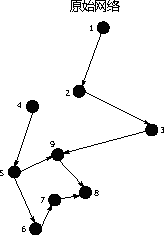
\includegraphics[width=5cm]{./figures/img/originalNetwork.pdf}
\caption{算法生成网络的示意图}
\label{fig:net}
\end{figure}
\subsection{算法时间复杂度分析}
从算法~\ref{alg:genegraph}~中可以看出,在循环内部的条件判断语句和对$N$的赋值语句的时间复杂度都为$O(1)$的,从前一部分的分析又知道\texttt{isLinkable($tr_i,tr_j$)}的时间复杂度为$O(1)$。对于$Tr$中的每一个出行$tr_i$,我们都将其与索引在$i$之后的所有出行$Tr(i+1:)$进行判断,设$m = |Tr|$,则总共判断了$\frac{m(m-1)}{2}$次,所以以上算法的时间复杂度为$O(\frac{m(m-1)}{2})$。由于想要得到完整的网络,我们必须对$Tr$中的所有出行组成的所有出行对进行分析,由于有$m$个出行数据,我们就必须进行至少$\frac{m(m-1)}{2}$次比较。故此算法的时间复杂度只能为$O(\frac{m(m-1)}{2})$。

\section{求解所需最少车辆算法设计与分析}
前两部分我们分别介绍了如何判断两个出行之间是否可以在图中有一条有向边,以及根据此判断标准生成完整的网络。在这一部分,我们将介绍如何将原始的网络,根据问题的实际意义,以及数据的意义,转化成二分网络,之后再介绍如何将寻找最少车辆服务所有出行的问题,建模成最小路径覆盖问题,并最终转化成二分网络中的最大匹配问题。最后,我们利用著名的求解二分图上最大匹配的Hopcroft-Karp算法,求解得到需要的最少车辆数。
\subsection{问题为路径覆盖问题}
下面我们将引入一些定义和定理,从而严格的说明,在已知所有的出行数据时,寻找最少的车辆数以服务所有出行的问题,实际上就是在我们已经得到的所有出行数据形成的网络上的路径覆盖问题(path cover)。
\begin{definition}[路径]
在一个有向网络$G = (N, E)$中,$G$中的一个路径$P$为由有向边组成一个序列$\{e_1 = (N_1^1, N_1^2),\cdots, e_k = (N_k^1,N_k^2)\}\in E$,使得$n_i^2 = n_{i+1}^1, i = 1,\cdots, k-1$,路径$P$中的节点集合为$N(P) = \bigcup_{i=1}^k n_i^1$。路径$P$的长度即为$k$。
\end{definition}

\begin{definition}[路径覆盖]
在一个有向网络$G = (N, E)$中,$G$中的一个无共同节点的路径覆盖,是一个在$G$上的一组路径$\{P_1, \cdots, P_h\}$的集合,并且使得$\bigcup_{i=1}^h N(P_i) = N, N(P_i)\cap N(P_j) = \emptyset, i\neq j$。
\end{definition}
\par
需要特别指出的是,在路径覆盖中,我们认为一个单独的节点为一个路径长度为0的路径。基于以上的定义,我们可以通过如下的定理和推论证明原问题等价于路径覆盖问题。
\begin{theorem}\label{theo:path}
对于网络$G = (N, E)$上的一个路径覆盖$\mathcal{C} = \{P_1,\cdots, P_h\}$,所有的出行都可以被服务到。
\end{theorem}

\begin{proof}
对于网络$G = (N,E)$上的一个路径$P= \{e_1 = (n_1^1, n_1^2),\cdots, e_k = (n_k^1,n_k^2)\}$,根据我们生成网络上边的算法,可以知道$n_1^1,n_1^2$(记为$tr_1,tr-2$),两个出行可以被同一辆车服务,并且,按照我们的判别条件,服务$tr_1$的车一定能在$t_2^o$之前到达$I_2^o$接到乘客。因此,出行$tr_2$的出发时间和达到时间没有延误。故和$n_1^2$有边的$n_2^2$所代表的出行不会延误,即车可以在指定时间之前到达出发地接到$n_2^2$代表的出行的乘客。同时,因为在我们的判别条件中,只有一个或者两个乘客的出行只能被二座车服务,有三个或者四个乘客的出行只能被四座车服务,$n_1^1,n_1^2,n_2^2$的乘客数量也都在同一类中(或者都只有一个或者两个乘客,或者都有三个或者四个乘客)。以此类推,路径$P$中的所有$N(P)$个乘客都可以被同一辆车准时服务到,没有出行的延迟。因此,对于路径覆盖$\mathcal{C}$,所有的出行都可以被不同的车服务到。
\end{proof}
\par
以上我们证明了,网络$G = (N, E)$上的一个路径覆盖,如果我们以一辆车代表一个路径,则$G$上的一个路径覆盖即是可以服务所有出行的一个可行解。接下来,我们证明任意一个原问题的可行解,即一个车辆的分配使得所有出行都被服务到,都对应了$G$上的一个路径覆盖。
\begin{theorem}\label{theo:origin}
对于所有出行的一个车辆分配,在网络$G = (N, E)$中,都存在一个路径覆盖$\mathcal{C} = \{P_1,\cdots, P_h\}$。
\end{theorem}
\begin{proof}
记$T$为所有被分配的车辆的集合,$p_t = \{tr_1,\cdots, tr_{k_t}\}, \forall t \in T$为每辆车所被分配的出行的集合,并且不失一般性的,我们假定车辆$t$即按照$tr_1,\cdots,tr_{k_t}$的顺序接送出行,如图~\ref{fig:pathproof}~所示。则由于$tr_1,tr_2$之间满足函数\texttt{isLinkable}的判别条件,所以如果将$tr_1,tr_2$都对应为网络中的一个节点,则它们之间有一条边,以此类推。所以如果将$p_t$中的所有出行都对应于网络上的节点,则$P_t = \{e_1 = (n_1^1, n_1^2),\cdots, e_{k_t} = (n_{k_t}^1, n_{k_t}^2)\}$为$G$中的一条路径,并且$P_t$中的每一个节点都代表了一个被服务的出行,其中$n_1^1$代表$tr_1$,$n_i^2, n_{i+1}^1$代表$tr_{i+1}, i = 1,\cdots, k_t$。将所有$P_t$这样的路径组合成一个路径覆盖$\mathcal{C} = \{P_1,\cdots, P_t\}$,则所有出行都在网络的节点中,所有的出行都被服务到。
\end{proof}
\begin{figure}
\centering
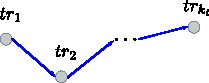
\includegraphics[width = 10cm]{./figures/img/pathproof.pdf}
\caption{车辆按照顺序接送}
\label{fig:pathproof}
\end{figure}
\par
从以上的分析中,可以知道寻找原问题的最优解,即找到最少的车辆服务所有的出行,等价于,在网络$G = (N,E)$中找到最少的路径覆盖,覆盖网络中所有的节点,并且不同的路径之间没有重合的节点。这是因为根据定理~\ref{theo:path}~,可以知道原问题所需的最少车辆数小于网络中的最少路径覆盖数,根据定理~\ref{theo:origin}~,可以知道网络中的最小路径覆盖数小于原问题中的最少车辆数。
\begin{figure}
\centering
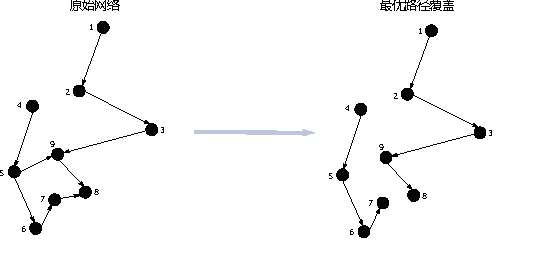
\includegraphics[width = 15cm]{./figures/img/pathcover.pdf}
\caption{在网络中找到最优路径覆盖}
\end{figure}

\subsection{将网络转化成二分网络}
在一个一般的有向网络中,我们并不能将其转换成二分网络。但是在本问题中,由于每次出行,我们都有其出发的交叉路口编号,以及达到的交叉路口的编号,我们可以通过将一个出行分为两个节点,即将出行在网络中所对应的节点,拆分为两个节点,分别代表出行的出发节点和出行的到达节点。这样所有出行的出发节点和到达节点分别组成了节点集合,这两个节点集合就是二分图中的两个节点集合,即原始的网络被转换成了一个二分网络。算法~\ref{alg:convert}~展示了上述的思路。为了更加严格说明此方法,我们将引入一些定义,定理和证明。

\begin{algorithm}[htbp]
\SetAlgoLined
\SetKwInOut{Input}{Input}\SetKwInOut{Output}{Output}
\caption{convertToBipartite($G = (N,E)$)}
\label{alg:convert}
\BlankLine
$G_b \leftarrow \emptyset$\;
$N_b \leftarrow \emptyset$\;
$E_b \leftarrow \emptyset$\;
\For{$v$ in $N$}{
  $tr_i\leftarrow$$v$所代表的出行\;
  $v_o^i\leftarrow$$tr_i$的出发交叉路口对应的节点\;
  $v_d^i\leftarrow$$tr_i$的到达交叉路口对应的节点\;
  $N_b\leftarrow N_b \cup \{v_i^o,v_i^d\}$\;
}
\For{$e = (u,v)$ in $E$}{
  $tr_i\leftarrow u$所代表的出行\;
  $tr_j\leftarrow v$所代表的出行\;
  $E_b\leftarrow E_b\cup \{(v_i^d, v_j^o)\}$\;
}
return $G_b = (N_b, E_b)$\;
\end{algorithm}

\begin{definition}[二分图]
对于图$G = (N,E)$,若$G$可以被划分成两个节点集合$S,T$,使得$S\cup T = N, S\cap T = \emptyset$,并且$\forall u, v\in S, (u,v)\notin E,(v,u) \notin E$,$\forall u, v\in T, (u,v)\notin E,(v,u) \notin E$,则$G$称为二分图。
\end{definition}
\par
图~\ref{fig:biparEx}~为一个二分图的示例。
\begin{figure}
\centering
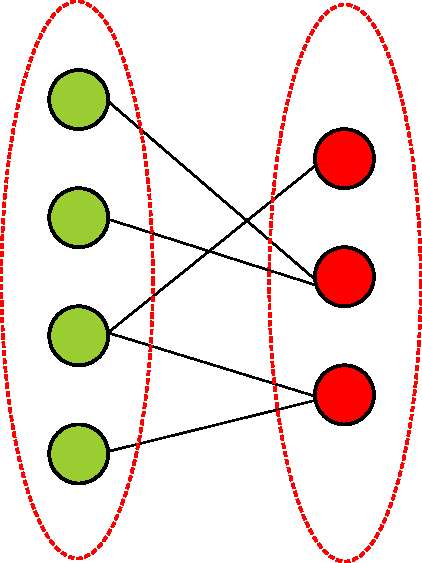
\includegraphics[width = 5cm]{./figures/img/bipartiteGraph.pdf}
\caption{二分图示例}
\label{fig:biparEx}
\end{figure}
\par
根据二分图的定义,我们可以给出如下的定理,证明我们的算法得到的图的确是二分图。
\begin{theorem}
根据算法~\ref{alg:convert}~得到的图$G_b=(N_b,E_b)$为二分图。
\end{theorem}

\begin{proof}
我们将所有出发节点组成的集合记为$N_o$,所有到达节点组成的节点组成的集合记为$N_d$,即$N_o = \{v_i^o| \forall tr_i \in Tr\},N_d = \{v_i^d| \forall tr_i \in Tr\}$,则我们证明$N_o. N_d$构成了对$G_b$的一个划分,使得$N_o\cup N_d = N_b, N_o\cap N_d = \emptyset$,并且满足二分图定义中的其他条件。
\par
首先,$N_o\cap N_d = \emptyset$是显然的,因为一个为出发节点集合,一个为到达节点集合。从算法~\ref{alg:convert}~中又可以知道$N_b$中的节点即为所有出发节点和到达节点,所以$N_o\cup N_d = N_b$。
\par
对于$E_b$中的一个边$e$,根据算法~\ref{alg:convert}~,可以将$e$记为$e = (v_i^d, v_j^o)$,而$v_i^d \in N_d, v_j^o \in N_o$。由$e$的任意性知,网络$G_b$中的所有边都满足这样的条件,所以$G_b$为二分图。
\end{proof}
\par
图~\ref{fig:bipar}~展示了将原始一般有向网络转换为二分网络。
\begin{figure}
\centering
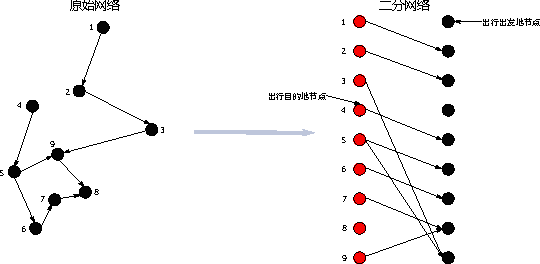
\includegraphics[height=8cm]{./figures/img/bipartiteNetwork.pdf}
\caption{將原始网络转化成二分网络}
\label{fig:bipar}
\end{figure}

\subsection{Hopcroft-Karp算法求解}
在一个一般的有向图中求解最小的路径覆盖是NP-hard的,即目前没有一个有效的多项式时间算法求解得到最优解。因此,在实际应用当中,对于交通网络而言,节点数量和边的数量都非常的大,想要求解得到最优解是几乎不可能的。但是,当有向图中没有有向圈时,存在一个高效的多项式算法求解得到最优解。无有向圈的有向图(或称为有向无环图,Directed Acyclic Network,简称DAG)的定义如下:
\begin{definition}[DAG]
一个有向图$G = (N,E)$称为是无有向圈的,如果$G$中不存在一条有向路径$P$,从$P$中一个节点$v$出发,沿着$P$的指向向前,会再次回到$v$。
\end{definition}
\par
根据以上定义,我们可以知道任何出行数据生成的有向图,都是无有向圈的,我们将其列为一个定理。
\begin{theorem}
根据全部出行数据$Tr$,以及判断两个出行是否可以被同一辆车服务的函数\texttt{isLinkable},生成的图$G = (N,E)$为DAG。
\end{theorem}
\begin{proof}
假设$P$为图$G$中的一个有向圈,并且我们可以不妨假设$P$的长度为2,因为长度为0和1的有向圈不存在,可以类似的证明长度大于2的有向圈不存在。
\par
设$P = \{(N_1, N_2), (N_2, N_1)\}$,则
\[
  t_1^d \leq t_2^o < t_2^d \leq t_1^o
\]
\par
但是,根据出行时间的意义,可以知道$t_1^d > t_1^o$,矛盾。
\par
这样我们就证明了$G$中不存在长度为2的有向圈,同样的可以证明,长度大于2的有向圈也不存在。
\end{proof}

\par
以上我们证明了,根据出行数据生成的网络为无有向圈的,因此可以在多项式时间复杂度的情形下求解最小的路径覆盖。接下来我们证明在二分图上求解最大匹配等价于在原始网络上求解最小路径覆盖。
\begin{theorem}
在$G_b = (N_b,E_b)$上的最大匹配$M$等价于在$G = (N,E)$上的最小路径覆盖。
\end{theorem}
\begin{proof}
假设$\mathcal{C} = \{P_1,\cdots, P_h\}$为$G$的最小路径覆盖,$\mathcal{M} = \{(u_1,v_1),\cdots, (u_s, v_s)\}$为$G_b$的最大匹配。
\par
由于$\mathcal{C}$为最小路径覆盖,故$h$为所有路径覆盖中最小的值。$\mathcal{C}$中共有$|N| - h$条边,为所有路径覆盖中的最大值。我们将$\mathcal{C}$中的边按照算法~\ref{alg:convert}~的方法对应到$G_b$中的边,则$\mathcal{C}$中的每一条边都对应了$G_b$中两个节点的匹配,即$\mathcal{C}$对应了$G_b$中的一个匹配,故$|\mathcal{M}| \geq |N| - h$。
\par
另一方面,对于$\mathcal{M}$中的一个匹配,两个节点分别属于不同出行,并且这两个出行满足\texttt{isLinkable}的条件,在$G$中有一条边。将$\mathcal{M}$中的匹配都对应到$G$中,则得到$G$中的一个边的集合$E^\prime$。
\par
在$E^\prime$中,没有两条边有共同的端点。否则,我们可以分两种情况讨论。
\par
两条边若有共同的到达端点,则在$G_b$中,它们对应了相同的在$N_o$中的节点,这与$\mathcal{M}$是一个匹配矛盾。
\par
两条边若有共同的出发端点,则在$G_b$中,它们对应了相同的在$N_d$中的节点,这与$\mathcal{M}$是一个匹配矛盾。
\par
所以$E^\prime$为$G$的一个路径覆盖,从而$ |\mathcal{M}|\leq N-h$。
\par
综上所述,$|\mathcal{M}| = N - h$,即求解$G$中的最小路径覆盖可以转换成求解$G_b$中的最大匹配。
\end{proof}

\par
在证明了上述结论之后,我们就可以利用在二分网络求解最大匹配的高效多项式时间算法,Hopcroft-Karp算法求解。下面我们具体介绍Hopcroft-Karp算法,为此,我们需要引入一些概念。
\begin{definition}[自由节点]
对于二分网络$G_b = (N_b, E_b)$,以及$G_b$上的一个部分匹配$\mathcal{M}$,一个节点$v\in N_b$是自由节点,如果$v$不是$\mathcal{M}$中任何一条边的端点。
\end{definition}

\begin{definition}[增广路]
对于$G_b = (N_b,E_b)$以及其上的一个部分匹配$\mathcal{M}$,一条路径$P$称为是增广路,如果$P$的起始节点为一个自由节点,并且$P$中的边为属于$\mathcal{M}$和不属于$\mathcal{M}$交替的,最后的终止节点也为一个自由节点。严格的说,$P = \{(s,v_1^1), (v_1^2, v_2^1),\cdots, (v_k^2, t)\}$,其中,$s,t$为自由节点,$v_i^1 = v_i^2, \forall i = 1,\cdots,k$,并且,当$i$为奇数时,$(v_i^2, v_{i+1}^1)\in \mathcal{M}$,$i$为偶数时,$(v_i^2, v_{i+1}^1)\notin \mathcal{M}$。
\end{definition}
\par
从以上定义中,我们可以推得$\forall i=1,2\cdots,k,v_i^1$不是自由节点,即只有$s,t$为自由节点。

\begin{theorem}
对$G_b = (N_b,E_b)$以及其上的一个部分匹配$\mathcal{M}$,$P$为$G_b$上的一个增广路,则$\mathcal{M},P$的对称差,$\mathcal{M}\oplus P$,是一个由$|\mathcal{M}|+1$个元素组成的匹配。
\end{theorem}

\begin{proof}
根据增广路的定义,设$P = \{(s,v_1^1), (v_1^2, v_2^1),\cdots, (v_k^2, t)\}$,则当$i$为奇数时,$(v_i^2, v_{i+1}^1)\in \mathcal{M}$,$i$为偶数时,$(v_i^2, v_{i+1}^1)\notin \mathcal{M}$,从而$\mathcal{M}\backslash P = \mathcal{M}\backslash \{((v_i^2, v_{i+1}^1))|i\makebox[3em]{为奇数}\}$;$P\backslash \mathcal{M} = \{(v_i^2, v_{i+1}^1)|i\makebox[3em]{为偶数}\}$。并且$|\mathcal{M}\backslash P| = |\mathcal{M}| - \frac{|P|-1}{2}, |P\backslash \mathcal{M}| = \frac{|P|+1}{2}$。所以$|\mathcal{M}\oplus P| = |\mathcal{M}|+1$。
\end{proof}
\par
由以上定理可以知道,在图中寻找增广路并且与匹配做对称差,就得到了一个严格更大的匹配。由于图中的节点和边的数量都是有限的,必定能在有限次寻找增广路之后得到最优解。Hopcroft-Karp算法的思想即是如此,不断地寻找增广路,并且与现在的部分匹配进行对称差,得到新的匹配,这个匹配是严格更大。重复此步骤,直到图中没有增广路了为止,此时的匹配就为最大的匹配,为最优解。
\par
我们将Hopcroft-Karp算法的伪代码展示如算法~\ref{alg:karp}。

\begin{algorithm}[htbp]
\SetAlgoLined
\SetKwInOut{Input}{Input}\SetKwInOut{Output}{Output}
\caption{HopcroftKarp($G_b = (N_b,E_b)$)}
\label{alg:karp}
\BlankLine
初始化匹配$\mathcal{M}\leftarrow \emptyset$\;
\While{True}{
  $\mathcal{P}\leftarrow \{P_1,P_2,\cdots, P_h\}$为图中的最大的增广路集合,并且$P_i\cap P_j=\emptyset, i\neq j$\;
  \uIf{$\mathcal{P}=\emptyset$}{
    break\;
  }
  \uElse{
    $\mathcal{M}\leftarrow \mathcal{M}\oplus (\bigcup_{i=1}^k P_i)$\;
  }
}
return $\mathcal{M}$\;
\end{algorithm}

\par
图~\ref{fig:maxMatch}~展示了Hopcroft-Karp算法的运行示意图。
\begin{figure}
\centering
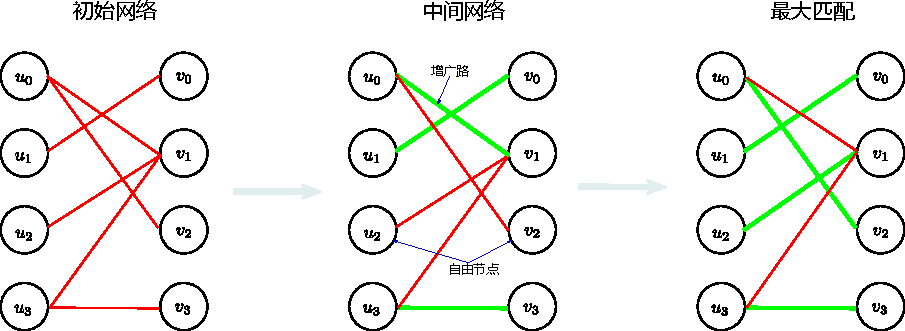
\includegraphics[width = 15cm]{./figures/img/maxMatch.pdf}
\caption{Hopcroft-Karp算法运行示意图}
\label{fig:maxMatch}
\end{figure}

\subsection{算法时间复杂度分析}
在以上的讨论中,共讨论了两个算法,一个是将原始有向图转换成二分图的算法~\ref{alg:convert}~和求解二分图中最大匹配的Hopcroft-Karp算法~\ref{alg:karp}。从算法~\ref{alg:convert}~中容易看出,主要的计算量在对每条边的循环操作,所以算法~\ref{alg:convert}~的时间复杂度为$O(|E|)$,生成的二分图的边的数量和原始图是相等的,节点的数量是原始图的两倍,即$|N_b| 2 |N|, |E_b| = |E|$。而Hopcroft-Karp算法的时间复杂度为$O(|E_b|\sqrt{|N_b|}) = O(|E|\sqrt{|N|})$。综上,这一部分的算法的总时间复杂度为$O(|E|\sqrt{|N|})$。


\section{实验结果}
我们使用在数据来源部分提到的数据进行的实际的编程计算。编程环境为Ubuntu 16.04 LTS @3.7GHz处理器,64GB RAM,编程语言为Python 3.6,使用了Numpy、Pandas、NetworkX进行数据处理,类和函数的定义编写,网络的生成和计算,使用了Multiprocessing库进行了并行计算。
